%----------------------------------------------------
% This is a preamble to the document
% The preamble of a document is where you place formatting information.
% It may look complicated but it is actually quite simple. 
% Comments have been added here to help you understand the meaning of the commands
%----------------------------------------------------
\documentclass[11pt,a4paper,final]{article}
\usepackage[latin1]{inputenc}


%----------------------------------------------------
% AMS Math package for math symbols
% Comment this line if you won't include math symbols in your document
%----------------------------------------------------
\usepackage{amsmath}
\usepackage{amsfonts}
\usepackage{amssymb}
%\usepackage{amsthm}
%\usepackage{makeidx}

%----------------------------------------------------
% Setup the geometry of the document
%----------------------------------------------------
\usepackage[left=2.50cm, right=2.50cm, top=2.50cm, bottom=2.50cm]{geometry}


%----------------------------------------------------
% Information for the title page
%----------------------------------------------------
\author{George Sithole}
\title{Mathematics for Geomaticians}
\date{28 January 2011}


%----------------------------------------------------
% PDF
% The pdftex package should be included if you intend
% to include graphics in your document.
% Comment the line below if you won't include graphics in your documnet.
%----------------------------------------------------
\usepackage[pdftex]{color,graphicx}


%----------------------------------------------------
% Paragraph formatting
% Change the following commands to affect paragraph
% formatting.
%----------------------------------------------------
\setlength{\parindent}{0pt}
\setlength{\parskip}{2ex}


%----------------------------------------------------
% New commands
%----------------------------------------------------
% ---------------------------------------------
% George Sithole 2011
% New commands used in this document
% ---------------------------------------------

% sigma 0
\newcommand{\sigmao}{\sigma_{0}}

% sigma 0 squared
\newcommand{\sigmaos}{\sigma^2_{0}}



% partial differential
\newcommand{\dydx}[2]
{
\frac{\partial #1}{\partial #2}
}


% ---------------------------------------------

% ATA
\newcommand{\ATA}[1]{A^T #1 A}

% ATA inverse
\newcommand{\ATAinv}[1]{(A^T #1 A)^{-1}}

% AAT
\newcommand{\AAT}[1]{A #1 A^T}

% AAT inverse
\newcommand{\AATinv}[1]{(A #1 A^T)^{-1}}


% BTB
\newcommand{\BTB}[1]{B^T #1 B}

% BTB inverse
\newcommand{\BTBinv}[1]{(B^T #1 B)^{-1}}

% BBT
\newcommand{\BBT}[1]{B #1 B^T}

% BBT inverse
\newcommand{\BBTinv}[1]{(B #1 B^T)^{-1}}


% vTPv
\newcommand{\vTPv}{v^{T}Pv}

% vTv
\newcommand{\vTv}[1]{v^{T} #1 v}

% xTx
\newcommand{\xTx}[1]{x^{T} #1 x}

% ---------------------------------------------
%            variance-covariance matrices
% ---------------------------------------------

% Sigma bb
\newcommand{\Sigmabb}{\Sigma_{bb}}

% Sigma ll
\newcommand{\Sigmall}{\Sigma_{ll}}

% Sigma LL
\newcommand{\SigmaLL}{\Sigma_{LL}}

% Sigma vv
\newcommand{\Sigmavv}{\Sigma_{vv}}

% Sigma ww
\newcommand{\Sigmaww}{\Sigma_{ww}}

% Sigma xx
\newcommand{\Sigmaxx}{\Sigma_{xx}}



% Pbb
\newcommand{\Pbb}{P_{bb}}

% Pll
\newcommand{\Pll}{P_{ll}}

% PLL
\newcommand{\PLL}{P_{LL}}

% Pvv
\newcommand{\Pvv}{P_{vv}}

% Pww
\newcommand{\Pww}{P_{ww}}

% Pxx
\newcommand{\Pxx}{P_{xx}}



% Qbb
\newcommand{\Qbb}{Q_{bb}}

% Qkk
\newcommand{\Qkk}{Q_{kk}}

% Qll
\newcommand{\Qll}{Q_{ll}}

% QLL
\newcommand{\QLL}{Q_{LL}}

% Qvv
\newcommand{\Qvv}{Q_{vv}}

% Qww
\newcommand{\Qww}{Q_{ww}}

% Qxx
\newcommand{\Qxx}{Q_{xx}}


%----------------------------------------------------
% Set equation numbering style
%----------------------------------------------------
\numberwithin{equation}{section}	% this will cause equation numbers to include section numbers


%----------------------------------------------------
% Bibliography style
% Comment this line if your document won't include references
%----------------------------------------------------
\bibliographystyle{plain}
%\usepackage{chicago}
%\citestyle{plain}
%\bibliographystyle{chicago}
%\bibliographystyle{plainnat}


% This is where you include the content of your document
\begin{document}

%----------------------------------------------------
% Change page numbering to roman numeral
%----------------------------------------------------
\pagenumbering{roman} 	% This command changes page numbering to roman numerals
\begin{center}
{\Huge University of Cape Town}
\linebreak \linebreak

{\LARGE School of Architecture and Planning and Geomatics}
\linebreak \linebreak

{\Large Geomatics Division}
\linebreak \linebreak


{\Large APG4003Z Project Proposal}
\linebreak

{\Large BSc Geomatics}
\linebreak \linebreak

\begin{center}

\includegraphics[width=0.5\linewidth]{includes/images/UCTcircular_logo1_CMYK.jpg}
\linebreak \linebreak
\end{center}

{\Large Designing a computer program that creates a 3D wire-frame model from a laser scan of the interior of a room}
\linebreak \linebreak

{\Large By: Tim Marsh}
\linebreak \linebreak

{\Large Supervisor: George Sithole}
\linebreak \linebreak

{\Large \today}

\end{center}
\addcontentsline{toc}{section}{Abstract}


\section*{Abstract}

The abstract goes here. The purpose of the abstract is to summarise the most important aspects of the document.

A reader will typically look at your document in this order

\begin{itemize}
\item Title

\item Abstract

\item Conclusion

\item Introduction

\item ... and so on
\end{itemize}


So your abstract should provide an overview of your paper emphasising on results and conclusions.


By the way above is an example of how to create a list.




%----------------------------------------------------
% Table of content
% Comment the lines below if you don't want a table of
% contents
%----------------------------------------------------
\pagebreak			 % This command causes a pagebreak
\tableofcontents	 % This command creates the table of contents


%----------------------------------------------------
% List of figures and list of tables
% Comment the lines below if you don't want a list of
% figures or a list of tables
%----------------------------------------------------
%\pagebreak	% This command causes a pagebreak
%\addcontentsline{toc}{chapter}{List of Figures}	% This command adds a line to the table of contents
%\listoffigures	% This command creates a list of figures

%\pagebreak
%\addcontentsline{toc}{chapter}{List of Tables} 
%\listoftables	% This command creates a list of tables


%----------------------------------------------------
% Change page numbering to arabic
%----------------------------------------------------
\setcounter{page}{1} % This command sets the page number to 1
\pagenumbering{arabic}	% This command changes page numbering to arabic


%----------------------------------------------------
% Chapters
%----------------------------------------------------
\label{MySection 1}
\section{Introduction}

In this section introduce the subject of the project. Provide a broad perspective on the subject area.


\label{MySubSection 1}
\subsection{Creating a sub section}
This is how you add a subsection.
The label command at the beginning of the subsection is used in referencing. (Look at the text)

To reference a section use the ref command. For example this is a reference to section \ref{MySubSection 1} (Look at the text)


\label{MySubSection 2}
\subsection{Creating another sub section}
This is how you add another subsection.


\label{MySubSubSection 1}
\subsection{Creating a sub sub section}
This is how you add a sub subsection. (Look at the text)

The label command at the beginning of the section is used in referencing. (Look at the text)

To reference a section use the ref command. For example this is a reference to the sub section \ref{MySubSubSection 1} (Look at the text)


\label{MySubSection 3}
\subsection{Adding Citations}

For convenience I have created a file called bibliography.bib. In this file are to be found the Bibtex references. If you want to add a reference to the document add it to this file. You may have to regenerate the bibtex references (press F11).

References are included in a document by using the bibliography command. For an example look at the file references.tex.
The style of referencing is set by the command bibliographystyle. For an example see the file main.tex.

To site a reference use the cite command. Here is an example \cite{Rie71}
Here is another example \cite{Ful83}.
The format of the citation is determined by the bibliiography style.


\label{MySubSection 1}
\subsection{Adding figures}

Here is you add figures. Notice the placement of the label and caption commands For simplicity I suggest that you use the Insert Figure Wizard (Under the Wizards menu).

\begin{figure} [hbtp]
\begin{center}
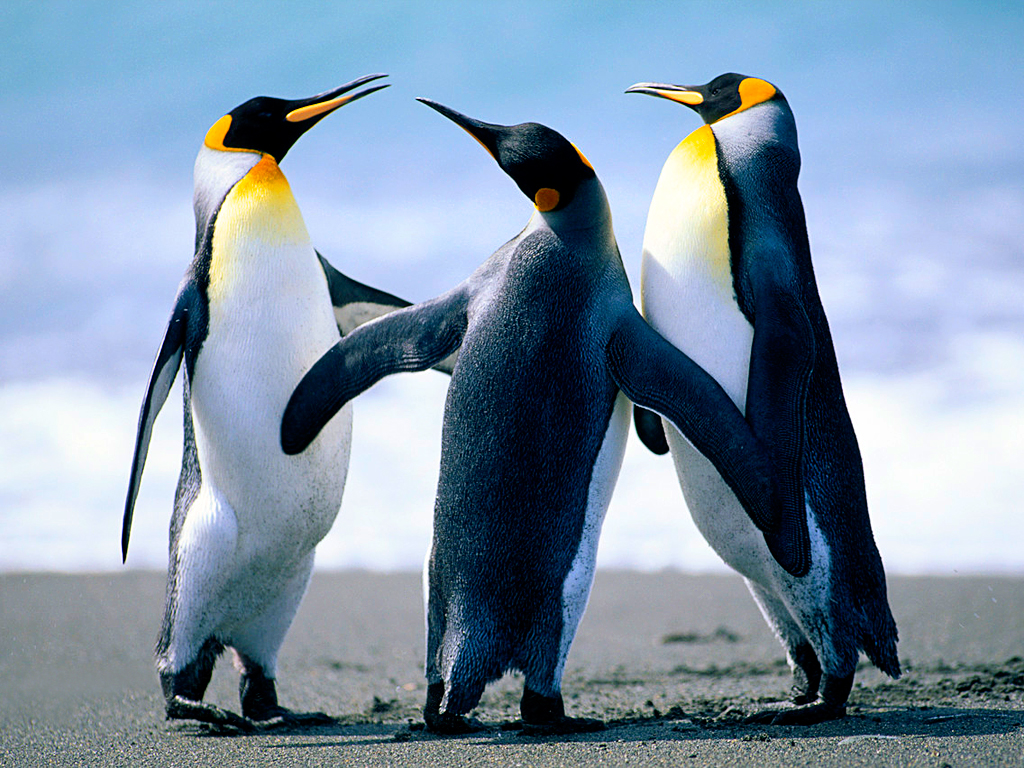
\includegraphics[width=12cm]{./images/Penguins}
\end{center}
\caption{Three student penguins having an important discussion, "What do you mean dude? Adele owns ..."}
\label{figPenguins}
\end{figure}

Here is how you reference the label \ref{figPenguins}


Here is another figure.

\begin{figure}[hbtp]
\centering
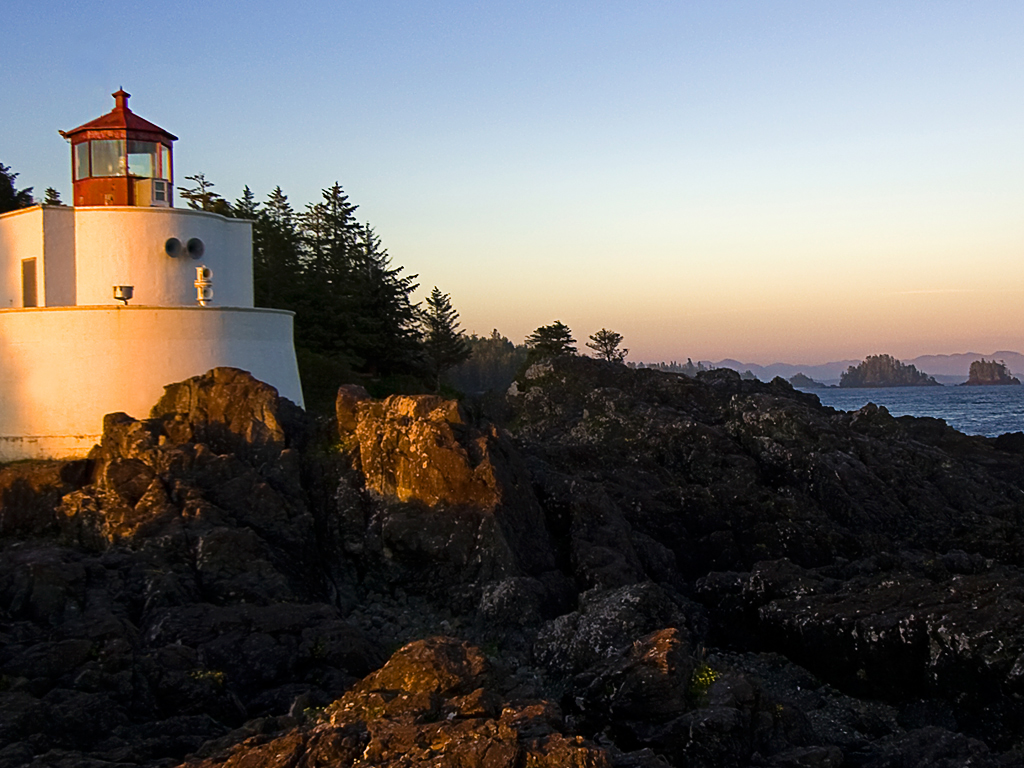
\includegraphics[width=12cm]{./images/Lighthouse}
\caption{Lighthouses ... only look good in pictures and wallpapers. Debate.}
\label{figLighthouse}
\end{figure}

Here is another reference the figure label \ref{figLighthouse}

In the next section we shall look at equations ...

\section{Previous Work}

Here is were you review previous work done in your field of research. The aim is to set the background against which your own work will be judged. Naturally you are expected to outline the state of the art.

\subsection{In-line equations}

In-line equations are equations embedded in your text. Here is an example of an in-line equation $\sigma^2 = \frac{\sum\limits_{i=1}^{n} (x_i - \bar{x})}{n}$. See how the equation runs with the text? All in-line equations are enclosed within dollar signs.

\subsection{Equations}

Here is a proper equations

\begin{equation}
\sigma^2 = \frac{\sum\limits_{i=1}^{n} (x_i - \bar{x})}{n}
\label{MyEquation1}
\end{equation}

Here is a reference to equation \ref{MyEquation1}




\section{Method}

In this section you describe the work that you will do.

\subsection{Objectives}

Here indicate the overall and specific objectives of your project.


\subsection{Questions}

Here discuss the questions that your project will have to answer in order to realise the objectives of the project.


\subsection{Proposed methods}

Here discuss how you will conduct the research. 

\begin{itemize}
\item What algorithms will you use?
\item What materials will you use?
\item What experiments will you conduct?
\end{itemize}
 
\section{Outcomes}

Here discuss the expected outcomes of your project.

\section{Schedule}

Here discuss the schedule of your project.

I suggest that you show the schedule using either a Gant Chart or a time line.
\include{conclusion}


%----------------------------------------------------
% Bibliography/References
%----------------------------------------------------
%----------------------------------------------------
% Add references to the table of contents
%----------------------------------------------------
\addcontentsline{toc}{section}{References} 


\bibliography{bibliography} % This command creates the bibliography

% The next line includes the whole bibliography in the document. This is not recommended.
%\nocite{*}	


\end{document}

